\documentclass[a4paper]{article}

\input ../header
\usepackage{minted}
\usepackage[np]{numprint}
\usepackage{lscape}
\usepackage{afterpage}
\usepackage{hyperref}

\setlength{\multicolsep}{2pt}

% Commandes pour cacher/révéler du texte facilement à l'aide d'un booléen
\usepackage{xstring}
\usepackage{ifthen}

\newboolean{reveal}
\setboolean{reveal}{true}

\newlength{\stextwidth} % une nouvelle longueur

\newcommand\x{6}

\newcommand{\guess}[1]{\ifthenelse{\boolean{reveal}}{{\color{red}#1}}{\settowidth{\stextwidth}{#1}\makebox[\stextwidth]{\dotfill}}}

\newcommand{\guessmath}[1]{\ifthenelse{\boolean{reveal}}{\textcolor{red}{#1}}{\settowidth{\stextwidth}{$#1$}\makebox[1.9\stextwidth]{\dotfill}}}

\newcommand{\guessmathbin}[1]{\ifthenelse{\boolean{reveal}}{\mathbin{\color{red}#1}}{\settowidth{\stextwidth}{$#1$}\makebox[2\stextwidth]{\dotfill}}}

\begin{document}

\title{La photographie numérique}

\pagestyle{empty}

\date{}
\author{}

\maketitle{}

\thispagestyle{empty}

\vspace*{-1cm}
\noindent\textbf{Activité 1}\hfill{}\textbf{Introduction}
\smallskip
\hrule
\medskip

Après avoir regardé la vidéo disponible sur Moodle, faire le test \og{}Tester ses connaissances\fg{}.

\bigskip

\noindent\textbf{Activité 2}\hfill{}\textbf{Quelques repères historiques}
\smallskip
\hrule
\medskip

Compléter chacun des paragraphes suivants :

\begin{itemize}
  \item \textbf{1827 -- La naissance de la photographie}\\
    En 1827, le Français \guess{Nicéphore Niépce} fixe pour la première fois une image (la vue depuis \guess{la fenêtre de sa maison}) sur un support. Il s'agit d'une plaque d'étain recouverte d'une sorte de gourdon qui réagit chimiquement avec \guess{la lumière}. L'image nécessite alors plusieurs \guess{jours} de pose. Mais la photographie ne naît officiellement que le 7 janvier 1839, jour de la présentation des travaux de \guess{Niépce} et de son partenaire \guess{Louis Daguerre} à l'Académie des sciences. Ce dernier remplace ensuite le goudron par de l'iodure d'argent, réduisant la pose à quelques dizaines de \guess{minutes} et ouvrant la voie à la photographie argentique.
  \item \textbf{1861 -- Le début de la photographie en couleur}\\
    La première photographie en couleur, prise par l'Anglais \guess{Thomas Sutton} et l'Écossais \guess{James Clerk Maxwell} en 1861, représente \guess{un ruban de tissu}. Elle est obtenue grâce à des prises de vue sous trois filtres différents : un filtre rouge, puis un vert et un bleu. Les plaques ont été développées et projetées sur un écran par trois projecteurs, chacun avec le même filtre coloré que celui utilisé lors de la prise de vue. L'image créée à partir des trois sources lumineuses colorées forme alors une image en couleur. Ce procédé s'inspire de la vision des couleurs de \guess{l'oeil humain}. Il est aujourd'hui à la base du codage RVB permettant à nos écrans d'afficher des millions de couleurs.
  \item \textbf{1957 -- La première photo numérisée}\\
    L'Américain \guess{Russell Kirsh} est l'un des premiers à numériser une photo en 1957. Sa résolution est très faible (l'image est donc peu détaillée), sa taille très petite ($5$ cm$^2$), et elle n'est pas en couleur mais en niveaux de \guess{gris}. Cette technologie a alors pour but de transférer une photo argentique papier vers un ordinateur pour la mettre en mémoire ou encore l'afficher à l'écran.
  \item \textbf{1969 -- L'invention du capteur CCD}\\
    En 1969, l'invention du capteur CCD (\guess{charged coupled device} en anglais) par le Canadien \guess{Willard Boyle} et l'Américain \guess{George E. Smith} révolutionne la photographie. On passe d'une pellicule photo à une plaque, composée de photosites, c'est-à-dire de petites cellules photoélectriques qui captent la lumière pour chaque pixel constituant l'image. C'est ce capteur qui tranforme ce que vous voyez à travers votre viseur en une imagen umérique.
  \item \textbf{1975 -- L'apparition des appareils photo numériques}\\
    Le premier appareil photo numérique, c'est-à-dire capable d'enregistrer une image sous forme de bits dans sa mémoire, est créé en 1975 pour la société américaine \guess{Kodak} par Steven J. Sasson. Cet appareil utilise un capteur CCD et enregistre des images en noir et blanc sur des cassettes, un processus qui prend 23 \guess{secondes}.
  \item \textbf{2000 -- Les téléphones portables avec appareil photo}\\
    Les premiers téléphones portables capables de prendre des photos ont été vendus par Sharp et \guess{Samsung} en 2000, démocratisant ainsi la photo numérique. Aujourd'hui, plus de \np{1000} milliards de photos sont prises chaque année par des smartphones, soit plus de $85\%$ des photos dans le monde.
\end{itemize}

\bigskip

Compléter également les paragraphes ci-dessous :

\begin{multicols}{2}
  \begin{enumerate}
    \item Je suis un physicien et mathématicien écossais. J'ai présenté la première photographie en vraie couleur.\\
      Je suis \dotfill
    \item Je suis une année durant laquelle la première photographie a été numérisée.\\
      Je suis \dotfill
    \item Je suis un composé chimique ouvrant la voie à la photographie argentique.\\
      Je suis \dotfill
    \item Je suis un composant transformant ce qui est perçu par notre oeil en image numérique.\\
      Je suis \dotfill
  \end{enumerate}
\end{multicols}

\bigskip

Réaliser une frise chronologique, puis la déposer au format PDF sur Moodle. Le nom du fichier déposé sera au format: 

\begin{center}
  \verb|[Classe]_[NOM]_[Prénom]_frise-photographie-numerique.pdf|,
\end{center} 

par exemple:

\begin{center}
  \verb|Seconde-15_RICARD_Louis_frise-chronologique.pdf|.
\end{center}

%\bigskip
%
%\noindent\textbf{Activité 3}\hfill{}\textbf{Photographie argentique, photographie numérique}
%\smallskip
%\hrule
%\medskip
%
%Un texte à compléter permettant de répondre aux questions 1. et 2. ci-dessous se trouve sur Moodle. Compléter ce texte puis noter les idées importantes sur cette feuille.\\
%Répondre à la question 3.
%
%\begin{enumerate}
%  \item Comparer la vitesse d'évolution des technologies de la photographie argentique avec celles de la photographie numérique.\rep{8}
%  \item Indiquer quelques différences fondamentales entre une photographie argentique et une photographie numérique.\rep{8}
%  \item Que change le capteur CCD pour la photographie ?\rep{8}
%    % Une photographie est désormais sous la forme de bits, des 0 et des 1, que l’on peut stocker
%    % dans des machines. Elle devient une information dématérialisée que l’on peut transmettre
%    % comme n’importe qu’elle autre information, par exemple sur un réseau d’ordinateurs.
%\end{enumerate}
%
%\bigskip
%
%
%\noindent\textbf{Activité 4}\hfill{}\textbf{L'oeil et le capteur photographique}
%\smallskip
%\hrule
%\medskip
%
%\begin{enumerate}
%  \item Compléter le texte du document 1, puis le schéma du document 2.
%    \begin{multicols}{2}
%      \textbf{Document 1 -- De l'oeil au cerveau}\\
%      Les rayons lumineux sont projetés au fond de l'oeil sur la \guess{rétine}. Celle-ci comprend des cellules sensibles à la lumière : les \guess{cônes}. Certains cônes perçoivent la couleur rouge, d'autres la couleur verte et d'autres la couleur bleue. Les cônes sensibles au vert sont les plus présents chez l'être humain. Ils transforment l'énergie lumineuse en impulsion électrique. Cette impulsion est transmise au cerveau par l'intermédiaire du nerf optique. La couleur est ensuite reconstituée par le cerveau par addition du rouge, du vert et du bleu.
%
%      \begin{center}
%	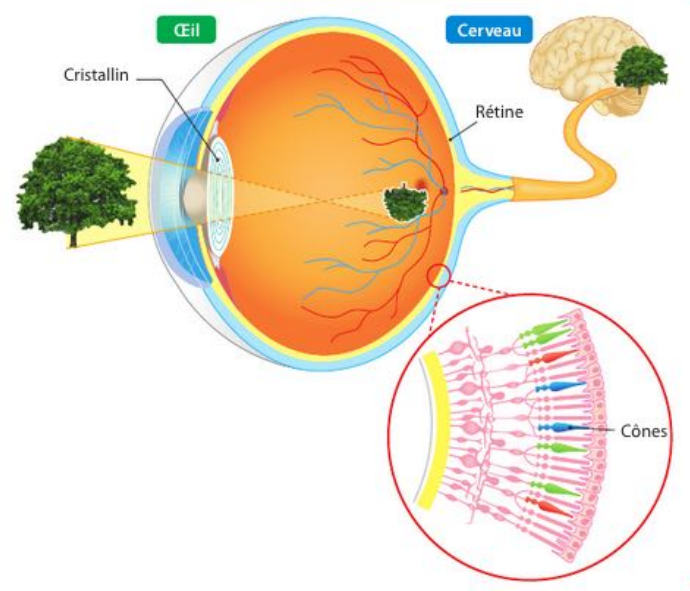
\includegraphics[width=8cm]{vision_humaine.png}
%      \end{center}
%    \end{multicols}
%
%    \pagebreak
%
%    \begin{multicols}{2}
%      \textbf{Document 2 -- Capture d'une image}\\
%      Les rayons lumineux entrent dans l'appareil photographique par l'objectif et sont projetés sur le capteur. La mesure de l'intensité lumineuse est transformée en données numériques avant d'être stockées dans la carte mémoire de l'appareil. Ces données permettent l'affichage de l'image sur un écran LCD.\columnbreak
%
%      \begin{center}
%	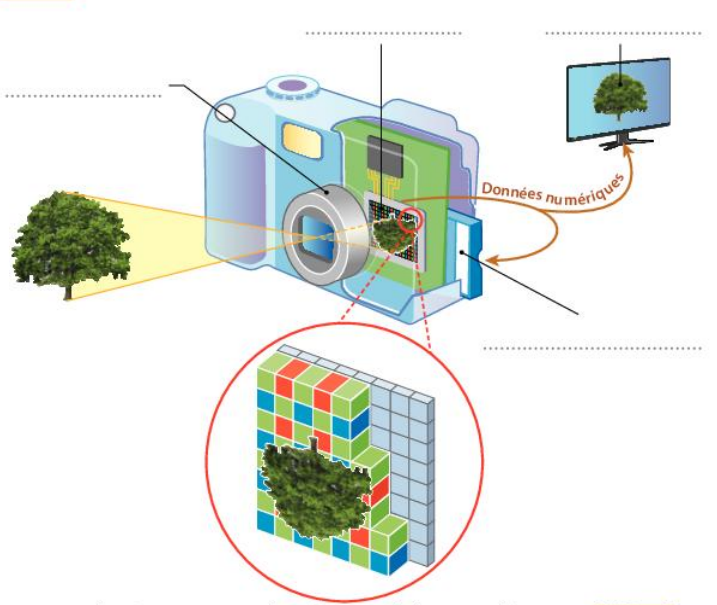
\includegraphics[width=8cm]{capture_d_une_image.png}
%      \end{center}
%    \end{multicols}
%  \item Comparer la capture d'une image par un oeil humain et un appareil photo (compléter le texte ci-dessous) :
%
%    L'appareil photo et l'oeil humain capturent la lumière de la même manière :
%    \begin{itemize}
%      \item la lumière passe à travers le \guess{cristallin} pour l'oeil et \guess{l'objectif} pour l'appareil photo ;
%      \item l'image est envoyée au fond de l'oeil sur \guess{la rétine} ou sur \guess{le capteur} pour l'appareil photo ;
%      \item la lumière est mesurée par \guess{les cônes} dans l'oeil et par \guess{les photosites} dans l'appareil photo (les mêmes couleurs sont mesurées : \guess{rouge}, \guess{vert} et \guess{bleu} ;
%      \item le message est ensuite envoyé au \guess{cerveau} ou jusqu'à la \guess{carte mémoire} et \guess{l'écran}.
%    \end{itemize}
%  \item Le document ci-dessous explique le fonctionnement d'un capteur photographique :
%    \begin{multicols}{2}
%      \textbf{Document 3 -- Fonctionnement d'un capteur photographique}\\
%      Le capteur photographique de l'appareil photo est composé de cellules sensibles à la lumière (on parle de cellules photosensibles) : les photosites. Ces cellules sont recouvertes de filtres colorés ne laissant passer que les rayons d'une seule couleur : rouge, vert ou bleu (2 verts, 1 bleu et 1 rouge par carré). Elles mesurent l'intensité lumineuse des rayons rouges (R), des rayons verts (V) et des rayons bleus (B). La définition d'un capteur est le nombre total de photosites.
%
%      \begin{center}
%	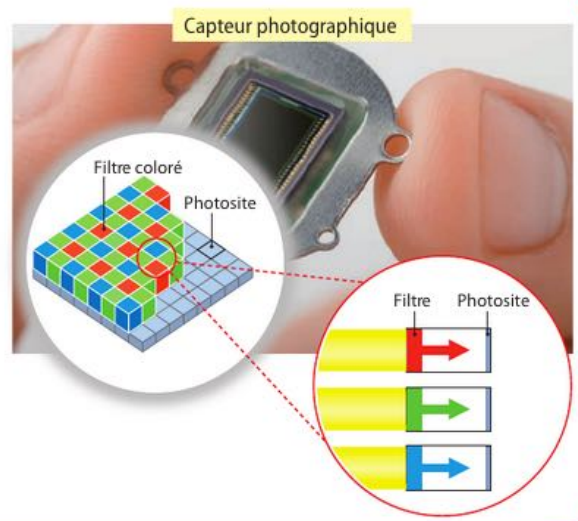
\includegraphics[width=8cm]{capteur_photographique.png}
%      \end{center}
%    \end{multicols}
%
%    Comparer la structure de la rétine d'un oeil et celle d'un capteur photographique (compléter le texte ci-dessous) :
%
%    La rétine est constituée de \guess{cônes} qui sont des cellules sensibles à la lumière bleue, verte ou rouge. De la même manière, le capteur de l'appareil photo est constitué d'éléments sensibles à la lumières : \guess{les photosites}. Comme on place des filtres colorés devant ces photosites, les rayons bleus, verts et rouges sont mesurés. Il y a plus de cônes sensibles au \guess{vert} et plus de photosites avec des filtres \guess{verts}.
%\end{enumerate}
%
%\pagebreak
%
%\noindent\textbf{Activité 5}\hfill{}\textbf{Les pixels d'une image}
%\smallskip
%\hrule
%\medskip
%
%\begin{enumerate}
%  \item Compléter le texte ci-dessous :
%    \begin{multicols}{2}
%
%      \begin{center}
%	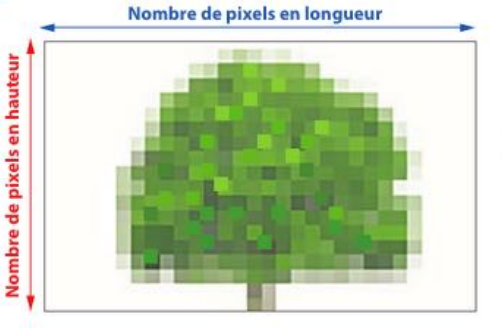
\includegraphics[width=8cm]{pixels_d_une_image.png}
%      \end{center}
%
%      \vspace*{12mm}
%
%      \textbf{Document -- Les pixels d'une image}\\
%      Après la capture d'une image, les données de couleurs sont enregistrées sous la forme d'un \og{}tableau de pixels\fg{}, c'est-à-dire de petits \guess{carrés} d'une couleur donnée. Une image est formée de millions de pixels : plus ils sont nombreux, plus l'image est précise.
%    \end{multicols}
%
%    \begin{multicols}{2}
%      \vspace*{5mm}
%    Dans l'appareil photo, il est possible de régler :
%    \begin{itemize}
%      \item la {\color{red}définition d'une photo}, soit le nombre total de pixels qui composent l'image ($\text{nombre de pixels en longueur}\times\text{nombre de pixels en hauteur}$, par exemple $\np{2048}\times\np{1152}$);
%      \item la {\color{red}résolution d'une photo}, soit le nombre de pixels par unité de longueur. Elle s'exprime en général en {\color{blue}pixels par pouce (ppp)}, ou en {\color{blue}\textit{dots per inch (dpi)}}.
%    \end{itemize}
%    \vspace*{10mm}
%
%    \begin{center}
%      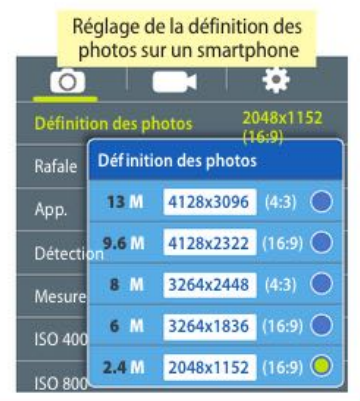
\includegraphics[width=5cm]{reglages_definition_sur_smartphone.png}
%    \end{center}
%    \end{multicols}
%
%    On pourra donc retenir la formule suivante :
%
%    \[\text{résolution (en ppp)} = \dfrac{\text{définition (en pixels)}}{\text{dimension (en pouces)}}\]
%
%    ($1$ pouce = $2,54$ cm)
%
%  \item Sur la capture précédente, quel réglage permet d'obtenir des photos de meilleure qualité ?
%  \item Expliquer la valeur \verb|9.6M|.
%  \item Que représentent la définition du capteur et la définition d'une photo ? Le nombre de pixels de la photo est-il nécessairement égal au nombre de photosites du capteur ? (compléter le texte ci-dessous)
%
%    \smallskip
%
%    La définition du capteur est le nombre de \guess{photosites}. La définition de la photo est le nombre de \guess{pixels} de l'image. Ces deux nombres ne sont pas forcément égaux car il est possible de diminuer la définition de la photo enregistrée dans les réglages de l'appareil. Le nombre de pixels de l'image est toujours \guess{inférieur ou égal} au nombre de photosites du capteur.
%  \item Un écran de smartphone mesure $6,4$ pouces de hauteur et $3,6$ pouces de largeur. Sa définition est de $\np{1920}\times \np{1080}$. Quelle est la résolution de cet écran ?
%  \item Les photos de Raphaël vont être exposées en galerie. L'établissement lui demande des fichiers pour réaliser des impressions aux dimensions de $50,8\times 33,87$ cm avec une résolution de $300$ dpi. Quelle définition minimale devront avoir les fichiers de Raphaël ?
%    \pagebreak
%  \item Voici ci-dessous une partie des caractéristiques techniques de l'iPhone 12 Pro :
%
%    \begin{multicols}{2}
%      \vspace*{1cm}
%    Pour calculer la résolution de $460$ ppp, le constructeur a tout d'abord déterminé le \og{}nombre de pixels situés sur la diagonale\fg{} de l'écran.
%    \begin{enumerate}
%      \item Retrouver ce nombre de pixels.
%      \item Retrouver alors la résolution annoncée.
%    \end{enumerate}\vspace*{6cm}\columnbreak
%    \begin{center}
%      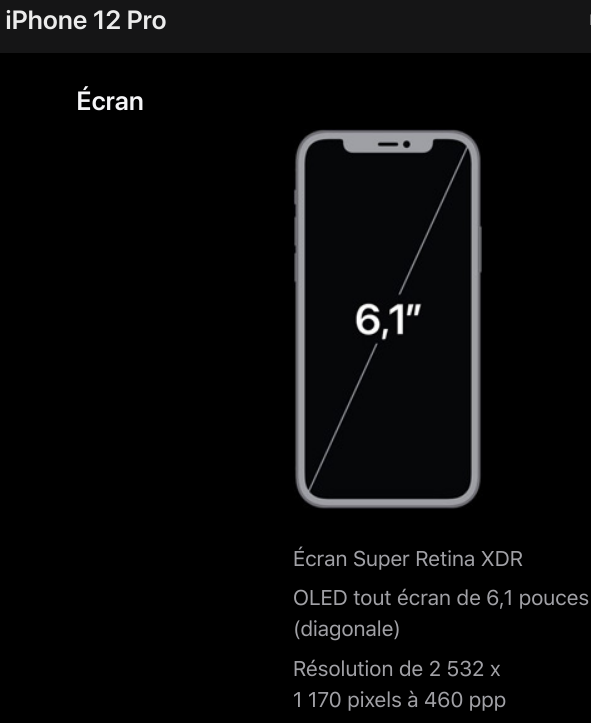
\includegraphics[width=8cm]{iphone_12_pro_resolution.png}
%    \end{center}
%    \end{multicols}
%  \item Déterminer la résolution de l'écran du Samsung S20 en utilisant la même méthode de calcul.
%\end{enumerate}
%
%\bigskip
%
%\noindent\textbf{Activité 6}\hfill{}\textbf{}
%\smallskip
%\hrule
%\medskip
%
%

\end{document}
